\documentclass[11pt,a4paper]{article}
\usepackage[utf8]{inputenc}
\usepackage[italian]{babel}
\usepackage{amsmath}
\usepackage{amsfonts}
\usepackage{amssymb}
\usepackage{graphicx}
\usepackage{minted}
\usepackage{enumitem}
\usepackage{tikz}
\usetikzlibrary{automata, positioning, arrows}
\usepackage[left=2cm,right=2cm,top=2cm,bottom=2cm]{geometry}
\author{\Large Davide Grazzani}
\title{\Huge \Huge Progetto Reti Logiche}
\date{}
\begin{document}
    \maketitle
    \newpage

    \tableofcontents
    \newpage

    \section{Codifiche Convoluzionali e Introduzione al Progetto}
    Una codifica convoluzionale è un tipo di codifica utilizzata per la \textit{Forward Error Correction} (FEC) in sistemi di telecomunicazioni basati su canali monodirezionali. \\
    Quindi un codice generato da una codifica convoluzionale, detto anche codice convoluzionale, è un codice che trasforma ogni parola $P_1$ in una parola $P_2$. Definite $l_1 = lenght(P_1)$ e $l_2 = lenght(P_2)$ si definisce il rapoorto $l_1/l_2$ come \textit{tasso di trasmissione del convolutore} (rate); $l_2 \geq l_1$.\
    Inoltre la trasformazione è una funzione degli ultimi $k$ bit in entrata, $k$ è quindi la \textit{lunghezza dei vincoli} del codice.\\
    Lo scopo del progetto è quello di implementare un componente hardware, tramite l'utilizzo del linguaggio di specifica dello hardware VHDL, in grado di interfacciarsi con una memoria ram e di applicare una codifica convoluzionale con $rate = \frac{1}{2}$ e $k = 3$.
    \begin{figure}[h]
        \centering
        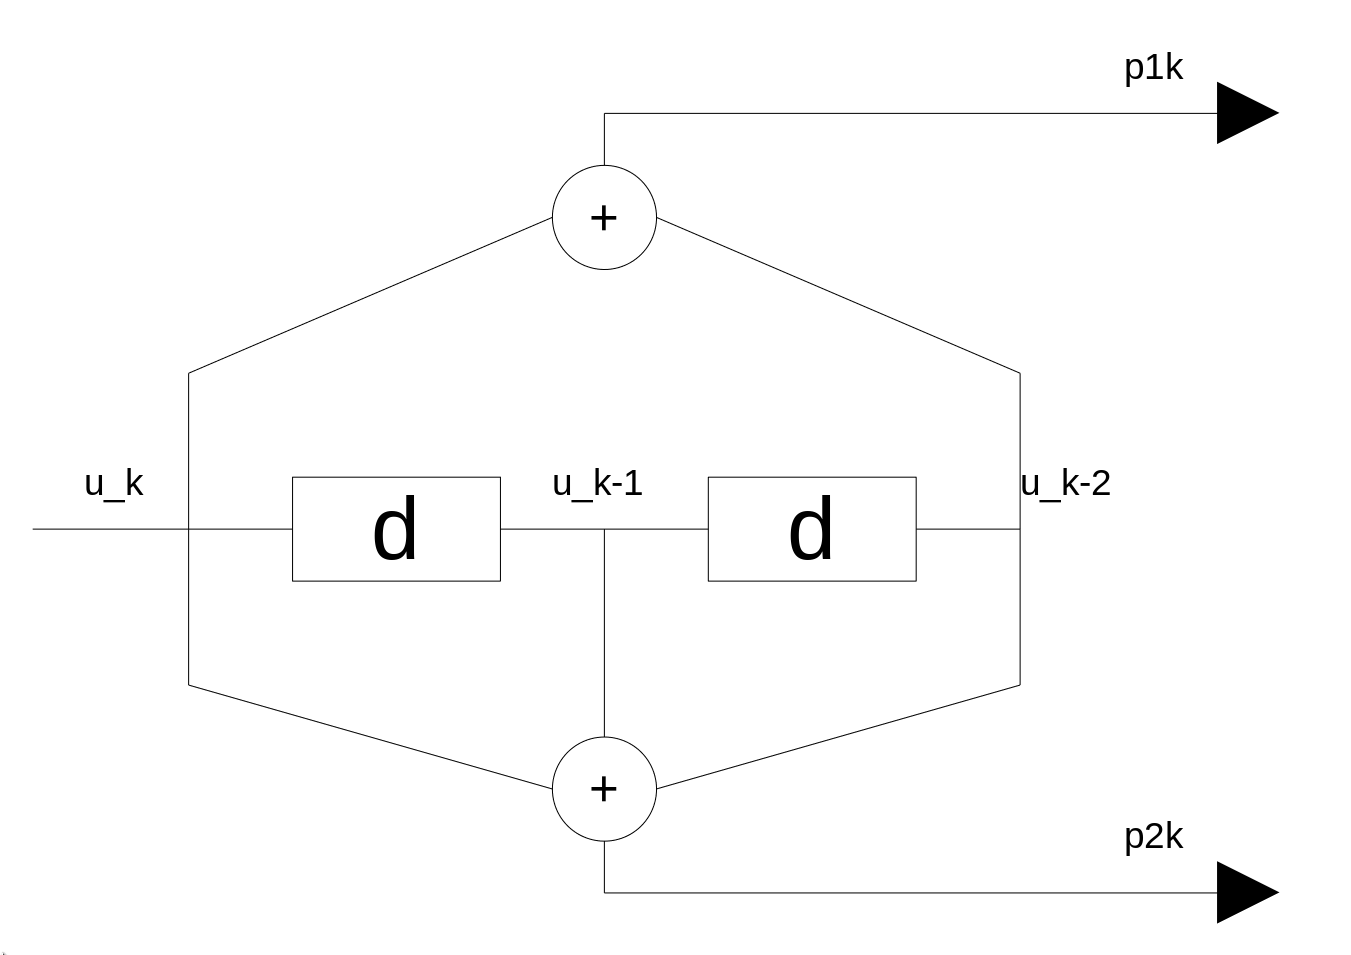
\includegraphics[width = 0.5\linewidth]{convolutore_image.png}
        \caption{Codificatore convoluzionale con $r = \frac{1}{2}$ e $k = 3$}
        \label{codificatore_convoluzionale_image}
    \end{figure}
    \subsection{Specifiche del progetto}
        Di seguito viene riportata l'interfaccia del modulo hardware da sviluppare, l'interfaccia della memoria ed infine alcune specifiche progettuali.
        \subsubsection{Interfaccia del progetto}
            \begin{minted}{vhdl}
            entity project_reti_logiche is
                port (
                    i_clk : in std_logic;
                    i_rst : in std_logic;
                    i_start : in std_logic;
                    i_data : in std_logic_vector(7 downto 0);
                    o_address : out std_logic_vector(15 downto 0);
                    o_done : out std_logic;
                    o_en : out std_logic;
                    o_we : out std_logic;
                    o_data : out std_logic_vector (7 downto 0)
                );
            end project_reti_logiche;
            \end{minted}
        \subsubsection{Interfaccia della memoria}
        TODO SISTEMARE QUESTA PARTE
        \subsubsection{Altri constrains progettuali}
        \begin{description}
            \item[Periodo di clock minimo richiesto] $clockPeriod_{req} = 100ns$
            \item[Ram] vedere   
        \end{description}
    \section{Architettura, approccio e scielte implementative}
        In questa sezione verrà descritta la \textit{FSM} del progetto seguita da un rapido overview sul codice presentato. Prima però vengono riportate alcune doverose considerazioni
        riguardanti il linguaggio di programmazione VHDL.
        \subsection{Considerazioni su VHDL}
            In questo progetto, durante la fase di progettazione e successivamente di sviluppo, non verrà preso mai in considerazione l'utilizzo del costrutto \textit{process} e di conseguenza
             di architetture di tipo \textit{behavioral} . Questa scelta implementativa, che si riflette sia in fase di sintesi che di implementazione, \underline{non è dovuta} al fatto che l'autore 
             del progetto creda che l'utilizzo di \textit{process} sia scorretto in qual si voglia forma o maniera; qui si vogliono riconoscere le potenzialità e le funzionalità implementative/strutturali 
             che ne derivano dall'utilizzo di quest'ultimi ma si vuole anche risaltare il maggior strato di astrazione portato da questo costrutto rispetto ad architetture \textit{dataflow} o \textit{structural} (aumento presumibilmente
             dovuto alle serializzazione di istuzioni che per natura fisica di un componente hardware dovrebbero essere paralle).\\
            È per il motivo sopra citato e per la non diretta corrispondenza tra codice scritto e struttura interna del sintetizzato hardware che in questo progetto sono state scartate implementazioni di tipo \textit{behavioral}.
        \subsection{Primo design della FSM}
            Tenendo conto delle considerazioni sopra fatte viene ora presentata la prima macchina a stati in grado già di soddisfare ampiamente requisiti di timing sia post sintesi sia post implementazione; viene discussa quest'ultima in 
            quanto alla base del design finale e da considerarsi design ottimale per periodi di clock $clockPeriod \approx [35,100] ns$.
            \subsubsection{Stati della macchina}
                \begin{figure}[h]
                    \centering
                    \begin{tikzpicture}[>=stealth',shorten >=1pt,auto,node distance=3cm,initial text =\texttt{Reset}]
                        \node[state, initial, initial where=left] (i)                    {$idle$};
                        \node[state]                              (r_wc) [right of=i]    {$r_{wc}$};
                        \node[state]                              (r)    [right of=r_wc] {$ r  $};
                        \node[state]                              (p_0)  [right of=r]    {$p_0 $};
                        \node[state]                              (p_1)  [right of=p_0]  {$p_1 $};
                        \node[state]                              (p_2)  [right of=p_1]  {$p_2 $};
                        \node[state]                              (p_3)  [below of=p_2]  {$p_3 $};
                        \node[state]                              (p_4)  [left of=p_3]   {$p_4 $};
                        \node[state]                              (p_5)  [left of=p_4]   {$p_5 $};
                        \node[state]                              (p_6)  [left of=p_5]   {$p_6 $};
                        \node[state]                              (p_7)  [left of=p_6]   {$p_7 $};
                        \node[state]                              (d)    [left of=p_7]   {$ d  $};
                        \path[->] (i)      edge [loop above] node {\texttt{start = '0'}} (i);
                        \path[->] (i)      edge              node {start = '1'}          (r_wc);
                        \path[->] (r_wc)   edge              node {}                     (r);
                        \path[->] (r)      edge              node {}                     (p_0);
                        \path[->] (p_0)    edge              node {}                     (p_1);
                        \path[->] (p_1)    edge              node {}                     (p_2);
                        \path[->] (p_2)    edge              node {}                     (p_3);
                        \path[->] (p_3)    edge              node {}                     (p_4);
                        \path[->] (p_4)    edge              node {}                     (p_5);
                        \path[->] (p_5)    edge              node {}                     (p_6);
                        \path[->] (p_6)    edge              node {}                     (p_7);
                        \path[->] (p_7)    edge              node {}                     (d);
                        \path[->] (d)      edge [loop below] node {$wc = 0$}             (d);
                        \path[->] (d)      edge              node {start = 0}            (i);
                        \path[->] (d)      edge              node {$wc \neq 0$}          (r);
                    \end{tikzpicture}
                    \caption{Primo design della \textit{FSM}}
                    \label{prima_fsm}
                \end{figure}
                con $wc$ definito come numero di parole ancora da codificare.
                \begin{description}[leftmargin = 0cm]
                    \item[Idle - $idle$ : ] stato della macchina iniziale dove questa attende che il segnale \texttt{i\_start} venga portato alto; una volta che ciò accade in questo stato vengono anche settati \texttt{o\_en = '1'} e \texttt{o\_address = 0} in modo tale da rendere il modulo pronto a ricevere il numero di parole dalla ram. Questo anche coincide con lo stato di reset della FSM.
                    \item[Read word count - $r_{wc}$ : ] stato della macchina dove viene settato il numero di parole da codificare.
                    \item[Read word - $r$ : ] stato della macchina adibito alla lettura della prossima parola da codificare. In particolare in questo stato vengono settati i valori valori di \texttt{o\_en = '1'} e \texttt{o\_address = '1'} in modo tale da leggere la parola da codificare in questo ciclo della FSM
                    \item[Process - $p_0 \rightarrow p_7$ : ] serie di 8 stati della macchina utilizzati per l'effettiva codifica della parola. Questi servono in particolare a ciclare sul singolo bit della parola considerata, oltre a contribuire alla sincronizzazione dei sottomoduli del progetto(descritto in maniera dettagliata più avanti). Espandiamo specificatamente:
                    \begin{itemize}
                        \item $p_0$ : in questo stato viene anche letta la parola richiesta precedentemente nello stato $r$.
                        \item $p_3$, $p_4$ : in questi stati vengono settati \texttt{o\_en = '1'} e \texttt{o\_we = '1'} in modo tale da poter parallelizzare la scrittura della parola in memoria con la sua effettiva computazione.
                    \end{itemize}
                    \item[Done - $d$ : ] stato della macchina che si dedica al controllo del numero di parole rimaste da codificare. Se il numero di parole è $\neq 0$ allora la FSM ritornerà alla stato $r$ altrimenti rimarrà in qiesto stato fintanto che \texttt{i\_start = '1'}.
                \end{description}
        \subsection{Design finale della FSM}
            Come precedentemente scritto la macchina sopra specificata superava i test bench per periodi di clock $clockPeriod \approx [15,100] ns$ nelle simulazione behavioral e post-sintesi ma falliva post-implementazione per $clockPeriod <\approx 35 ns$ dove le latenze dell'FPGA erano maggiori.\\
            Possibile soluzione sarebbe quella di aggiungere altri 2 stati così da poter mitigare i ritardi dovuti alla lettura della memoria. Vengono quindi qui sotto riportate delle semplici, seppur doverose, analisi in termini di tempo e di spazio per poter giustificare il cambiamento delle stuttura della macchina a stati.
            \subsubsection{Analisi di trade-off spaziale}
                Considerando il numero di stati $numStati = 12$ e utilizzando la codifica binaria $log_2(numStati) \approx 3.6$ quindi si utilizzano 4 bit per la rappresentazione di tali stati. È facile verificare che l'aggiunta di 2 stati, quindi $numStati = 14$, non richiede allocamento aggiuntivo di memoria su FPGA.
            \subsubsection{Analisi di trade-off temporale}
                Essendo uno di questi 2 stati aggiuntivi eseguito solo una volta in fase di lettura del numero di parole contenuto in ram esso verrà trascurato perchè asintoticamente irrilevante. Tenendo in considerazione gli stati che vengono eseguiti in \textit{loop}, facendo riferimento alla figura \ref{prima_fsm} gli stati da $r$ a $d$, si ottine $numStati_{m1} = 10$ e $numStati_{m2} =numStati_{m1} + 1= 11$.\\
                Quindi perchè questa modifica alla FSM sia motivata si deve avere che 
                \begin{gather*}
                    numStati_{m1} * clockPeriod_{m1 \space min} > numStati_{m2} * clockPeriod_{m2} 
                \end{gather*}
                con $clockPeriod_{m1 \space min} = 35 ns$.\\
                Si ottiene che $clockPeriod_{m2} \leq 31.82 ns$, condizione che verrà poi verificata e discussa nella sezione riguardante i risultati sperimentali.
            \subsubsection{Nuova macchina a Stati}
                Vengono così aggiunti altri 2 stati :
                \begin{description}
                    \item[Wait word count - $w_{wc}$]
                    \item[Wait - $w$]  
                \end{description}
                entrambi adibiti alla mitigazione del ritardo dovuto alla lettura della memoria e alla propagazione di tale segnale in fase di implementazione.
                \begin{figure}[h]
                    \centering
                    \begin{tikzpicture}[>=stealth',shorten >=1pt,auto,node distance=3cm,initial text =\texttt{Reset}]
                        
                    \end{tikzpicture}
                    \caption{Design finale compatto della \textit{FSM} finale}
                    \label{seconda_fsm}
                \end{figure}
\end{document}